\documentclass[12pt]{article}
\usepackage[a4paper, top=1in, left=1in, right=1in, bottom=0.6in]{geometry}
\usepackage[utf8]{inputenc}
\usepackage{hyperref}
\usepackage{tikz}
\usepackage{float}
\usepackage{multirow}
\usepackage{pifont}
\usepackage{amsmath}
\usepackage{pdflscape}
\usepackage{amssymb}
\usepackage[backend=biber,style=numeric,sorting=none,sortcites,backref,hyperref]{biblatex}
\addbibresource{references.bib}

\makeatletter
\renewcommand\footnotesize{\scriptsize}
\makeatother

\newcommand{\citerel}{\overset{\mathit{cite}}{\rightarrow}}
\newcommand{\nociterel}{\overset{\mathit{cite}}{\nrightarrow}}

\title{Recommender System for Research Papers \newline\newline \small Group 17}
\author{
  Matthias Bergmann (12219019) \and Maximilian Herczegh (12306066) \and Alexander Scheucher (12113826) \and
    Patrick Ziegler (12303709)
}
\date{\today}

\begin{document}

\maketitle

\begin{abstract}
  With the ever growing amount of research papers being published, it becomes increasingly difficult for researchers to
  stay updated in their respective fields and discover relevant literature. To address this challenge, we propose the
  development and evaluation of a recommender system specifically designed to suggest relevant research papers based on
  abstract-style textual user queries. In particular, we aim to evaluate the performance of various pre-trained embedding
  models, fine-tuned variations and different retrieval techniques (such as the use of a separate model to re-rank
  approximate k-nearest results) in the context of recommending research papers. The recommender system will be evaluated
  using a large-scale dataset of research papers with query-positive-negative triplets derived from citation
  relationships.\\ Our overarching research question is: \emph{How well do different combinations of transformer-based
    embedding models and re-ranking models perform for research paper recommendation when evaluated on citation-based
    benchmarks?}
\end{abstract}

\begin{figure}[H]
  \centering
  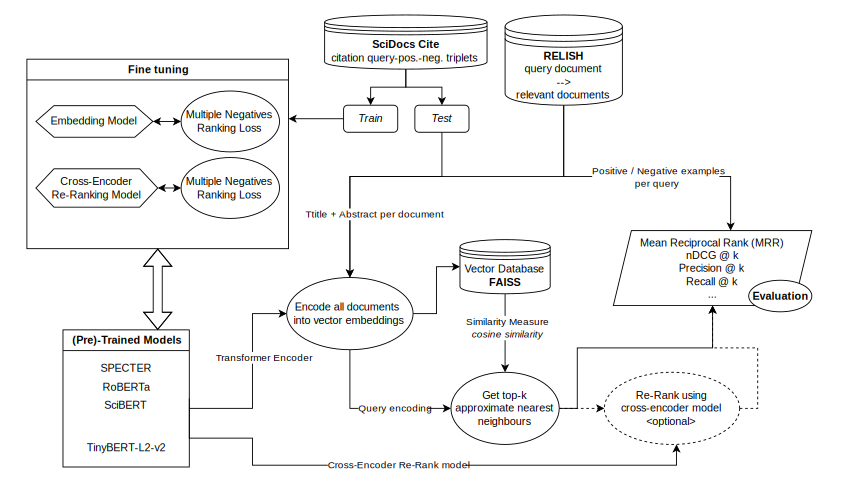
\includegraphics[width=\textwidth]{AIR_schematic_new.pdf}
  \caption{System schematic of the proposed paper recommender pipeline.}
  \label{fig:air-schematic}
\end{figure}

\newpage

\section{Introduction}

Using transformer-based embedding models for text representation and information retrieval has become increasingly
popular in recent years. In particular, models such as BERT~\cite{devlin-etal-2019-bert} and its variants have
demonstrated remarkable performance on embedding tasks. Furthermore, the task of recommending resesarch papers on a
given context has gained significant attention due to the growing volume of scientific literature. These systems aim to
assist researchers in discovering relevant papers efficiently and aim to improve upon traditional keyword-based search
methods. However, the lack of large-scale, high-quality datasets labeled for this task poses a significant challenge
for the development and evaluation of such recommender systems.

In this report, we evaluate how models fine-tuned on citation-based datasets perform in the context of recommending
research papers. We explore various combinations of embedding models and retrieval techniques, including the use of
re-ranking models to enhance the quality of the retrieved results.

\section{Related Work}

Cohan et al.~\cite{cohan-etal-2020-specter} introduced SPECTER, a model specifically designed for generating
document-level embeddings of scientific papers based on the titel and abstract. SPECTER is fine-tuned on a large corpus
of research papers using citation relationships as supervision signals. Singh et al.~\cite{Singh2022SciRepEvalAM}
created SciRepEval, a larger benchmark dataset with multiple tasks for evaluating and comparing scientific paper
representation models to address the reliance on citation-based supervision. This also includes
RELISH~\cite{brown2019large}, an expert annotated dataset for research paper recommendations.

Multiple pre-trained transformer-based models have been proposed for scientific text, such as
SciBERT~\cite{beltagy-etal-2019-scibert}. Furthermore, the use of small cross-encoders, such as
TinyBERT~\cite{jiao-etal-2020-tinybert}, for re-ranking retrieved documents has been shown to improve retrieval
performance~\cite{nogueira2019multi} in multiple domains.

We build upon these works and directly compare these existing fine-tuned models and cross-encoders for the task of
research paper recommendation within a unified framework.

\section{Experiments and Results}

\subsection{Datasets}

We are using the citation-triplets dataset from SciRepEval~\cite{Singh2022SciRepEvalAM} for fine-tuning our models.
This dataset is available as the \texttt{cite\_prediction\_new} split on
Huggingface~\footnote{\url{https://huggingface.co/datasets/allenai/scirepeval/viewer/cite_prediction_new}}. It contains
a train and evaluation test set, as used for the fine-tuning of SPECTER. Each sample in this dataset consists of a
query paper $\mathcal{P}^Q$, a positive paper $\mathcal{P}^+$ and a negative paper $\mathcal{P}^-$. Each paper contains
the title, an abstract and an unique corpus ID. The train set contains around 6.2 million samples, while the evaluation
set contains around 176k samples. On average, each query paper is part of 10 triplets. The positive paper is a paper
cited by the query paper, thus $\mathcal{P}^Q \citerel \mathcal{P}^+$. The negative papers consist of hard and easy
negatives. Hard negatives are papers that are not cited by the query paper, but are cited by a paper that is cited by
the query paper. Thus, a paper $\mathcal{P}^H$ is a candidate hard negative if there is an intermediate paper
$\mathcal{P}^I$ such that $\mathcal{P}^Q \citerel \mathcal{P}^I \citerel \mathcal{P}^H$ and $\mathcal{P}^Q \nociterel
  \mathcal{P}^H$. Easy negatives are randomly sampled papers that are not cited by the query paper.

To evaluate how a citation based recommender system transfers to real world recommendations we evaluate all our models
on the RELISH dataset~\cite{brown2019large} also available on
Huggingface~\footnote{\url{https://huggingface.co/datasets/allenai/scirepeval/viewer/relish}}. This dataset contains
expert annotated relevance judgements for research paper recommendations in the biomedical domain. It contains around
3k queries, each with 60 ranked documents on average. Each query and document contains the title and abstract.
Following the method of Brown and Yaoqi~\cite{brown2019large}, we consider documents marked \textit{relevant} as
positives and \textit{somewhat-relevant} and \textit{irrelevant} as negatives.

To ensure not data leakage occurs, we use the pre-existing split of the citation-triplets dataset and removed all
papers in the RELISH dataset from the training set of the citation-triplets dataset. This minimalizes data-leakage
between the train and evaluation sets and limis the amount of documents seen by the pre-trained models.

For fine-tuning, the training set of the citation-triplets is automatically downloaded from Huggingface, filtered and
converted to the correct format. Title and abstract are concatenated with a \texttt{[SEP]} token. This process is
automatically cached locally upon the first run. For evaluation on both datasets, all unique documents and
corresponding relevance judgements are extracted and converted to use with
\texttt{ir\_measures}\cite{ir-measures-2022}.

\subsection{Models and Methods}

The base models used for embedding generation are SPECTER~\cite{cohan-etal-2020-specter},
SciBERT~\cite{deka2021unsupervised} and a RoBERTa base model~\cite{reimers-2019-sentence-bert} as available on
Huggingface~\footnote{\url{https://huggingface.co/sentence-transformers/allenai-specter}}\footnote{\url{https://huggingface.co/pritamdeka/S-Scibert-snli-multinli-stsb}}\footnote{\url{https://huggingface.co/sentence-transformers/stsb-roberta-base-v2}}.
The cross-encoder used to re-rank the approximate nearest neighbor results is
TinyBERT-L2-v2~\cite{jiao-etal-2020-tinybert} from
Huggingface~\footnote{\url{https://huggingface.co/cross-encoder/ms-marco-TinyBERT-L2-v2}}. These models are all
implemnted using the \texttt{Sentence Transformers} library~\footnote{\url{https://sbert.net/}} and thus easily
interchangeable and fine-tunable.

\subsubsection{Fine-Tuning}

For testing the effect of fine-tuning, we fine-tune the RoBERTa base model on the citation-triplets dataset. We employ
a \texttt{MultipleNegativesRankingLoss}\cite{henderson2017efficient} loss function working directly on the
query-positive-negative triplets. This loss function maximizes the similarity between the query and positive sample,
while minimizing the similarity between the query and all other in-batch samples (negatives). This happens by embedding
each document separately and employing a cross entropy loss on the pairwise cosine similarities. Based on the available
GPU compute, we fine-tune for one epoch with a batch size of 40, 16-bit precision, learning-rate warmup and all other
parameters as default. The training is monitored using
\texttt{tensorboard}\footnote{\url{https://www.tensorflow.org/tensorboard}} to ensure no overfitting occurs.

The cross-encoder TinyBERT-L2-v2 is fine-tuned using the same parameters and loss funciton. However, this model
directly ouputs the similarity between the query and other documents. This is handled implicitly by the sentence
transformer library.

\subsubsection{Recommender System}
For each model combination, we create a recommender system that first encodes all documents in the evaluation set using
the embedding model. These embeddings are then stored in a FAISS~\cite{johnson2019billion} index to allow for efficient
approximate nearest neighbor search. For each query, we first retrieve the top-k nearest documents using the embedding
model. If a re-ranking model is used, we then re-rank these k documents using the cross-encoder model (by using the
predicted similarity between the query and each document). Finally, the top-k documents are returned as
recommendations. By default we use $k=20$ when evaluating a single embedding model and $k=30$ when using a re-ranking
model to ensure enough documents are available for re-ranking.

\subsection{Evaluation Metrics}

All obtained query-document rankings are evaluated using standard information retrieval metrics such as
\textit{Succes@k}, \textit{Mean Reciprocal Rank (MRR)}, \textit{Normalized Discounted Cumulative Gain (nDCG) @ k},
\textit{Mean Average Precision (MAP)}, \textit{Precision@k} and \textit{Recall@k} using the \texttt{ir\_measures}
library~\cite{zhu2004recall,jarvelin2002cumulated}. We employ query level bootstrapping with 1000 iterations to obtain
90\% confidence intervals for all metrics.

\section{Conclusion and Results}

Full evaluation results for all model combinations on both datasets and all metrics are shown in Appendix A
(Table~\ref{tab:metrics-relish} and Table~\ref{tab:metrics-scirepeval}). As can be seen in Figure

% Why MRR on relish is only where fine tuned reranker is better -> misaligned training objective (one positive many negatives)

\subsection{Limitations}
Although, we carefully cleaned the datasets to minimize data leakage, there is still a chance that some documents from
the RELISH dataset are present in the training set of the citation-triplets dataset or have been used during the
pre-training of the embedding models.

Due to limited computational resources and large dataset size, we could not employ hyper-parameter tuning or extensive
experiments on fine-tuning startegies. Thus, the fine-tuning process could be further optimized to improve performance.

Additionally, due to the limited availability of high-quality expert annotated datasets for research paper
recommendation, we could only evaluate on the RELISH dataset which is limited to the biomedical domain. Thus, the
generalization of our results to other scientific domains is limited.

Therefore, we suggest that future work should focus on obtaining larger and more diverse expert annotated datasets
based on real user interactions. Furhtermore, exploring more variations of fine-tuned models and different re-ranking
techniques could provide further insights into the optimal configurations for research paper recommendation systems.

% limitation of context length

\newpage

\begin{landscape}

\section*{Appendix A: All Metrics}

\begin{table}[h]
  \centering
  \renewcommand{\arraystretch}{1.25}
  \begin{tabular}{|l|l|c|c|c|c|c|}
  \hline
\textbf{Model} & \textbf{Reranker} & \textbf{MRR} & \textbf{nDCG@10} & \textbf{MAP} & \textbf{Recall@5} & \textbf{Recall@10}\\
\hline
\hline
\multirow{3}{*}{RoBERTa} & None & 51.9 (50.8--52.9) & 34.0 (33.2--34.7) & 13.8 (13.4--14.3) & 10.7 (10.3--11.1) & 17.1 (16.6--17.6)\\
\hline
 & TinyBERT & 62.4 (61.4--63.5) & 44.8 (44.0--45.6) & 20.1 (19.5--20.6) & 14.9 (14.4--15.4) & 22.4 (21.9--23.0)\\
 \hline
 & TinyBERT Fine Tuned & 64.2 (63.1--65.4) & 41.7 (40.9--42.5) & 18.5 (18.0--19.0) & 13.0 (12.6--13.5) & 20.5 (19.9--21.0)\\
 \hline
\hline
\multirow{3}{*}{RoBERTa Fine Tuned} & None & 64.4 (63.4--65.3) & 49.3 (48.5--50.1) & 25.0 (24.5--25.6) & 16.7 (16.2--17.2) & 26.7 (26.0--27.3)\\
\hline
& TinyBERT & 66.7 (65.7--67.7) & \underline{53.7 (52.9--54.4)} & \underline{30.7 (30.1--31.3)} & \textbf{17.9 (17.4--18.4)} & \textbf{29.2 (28.5--29.8)}\\
\hline
& TinyBERT Fine Tuned & \underline{69.2 (68.1--70.2)} & 48.8 (48.0--49.7) & 27.8 (27.3--28.4) & 15.2 (14.7--15.6) & 25.4 (24.9--26.0)\\
\hline
\hline
\multirow{3}{*}{SciBERT} & None & 61.3 (60.3--62.3) & 44.9 (44.1--45.8) & 21.3 (20.8--21.8) & 14.7 (14.3--15.2) & 23.8 (23.2--24.4)\\
\hline
& TinyBERT & 65.7 (64.7--66.7) & 51.2 (50.4--52.0) & 27.4 (26.8--28.0) & 16.9 (16.4--17.4) & 27.1 (26.5--27.7)\\
\hline
& TinyBERT Fine Tuned & 67.5 (66.5--68.6) & 46.7 (45.9--47.6) & 25.0 (24.4--25.5) & 14.3 (13.9--14.8) & 23.7 (23.2--24.3)\\
\hline
\hline
\multirow{3}{*}{SPECTER} & None & 65.9 (64.9--66.9) & 50.9 (50.2--51.7) & 25.7 (25.2--26.2) & 17.1 (16.7--17.6) & 27.1 (26.5--27.7)\\
\hline
& TinyBERT & 66.7 (65.7--67.7) & \textbf{54.1 (53.3--54.8)} & \textbf{31.0 (30.4--31.5)} & \underline{17.8 (17.2--18.3)} & \underline{29.1 (28.5--29.7)}\\
\hline
& TinyBERT Fine Tuned & \textbf{70.3 (69.3--71.4)} & 50.6 (49.9--51.4) & 28.9 (28.3--29.4) & 15.4 (15.0--15.8) & 26.1 (25.6--26.7)\\
\hline
\end{tabular}
  \caption{Evaluation results on the RELISH ranked recommendation dataset for all model combinations and selected metrics including the 90\% confidence interval. Best results per metric are \textbf{bolded}, second best are \underline{underlined}.}
  \label{tab:metrics-relish}
\end{table}

\begin{table}[h]
  \centering
  \renewcommand{\arraystretch}{1.25}
  \begin{tabular}{|l|l|c|c|c|c|c|}
  \hline
  \textbf{Model} & \textbf{Reranker} & \textbf{MRR} & \textbf{nDCG@10} & \textbf{MAP} & \textbf{Recall@5} & \textbf{Recall@10}\\
  \hline
  \hline
  \multirow{3}{*}{RoBERTa} & None & 41.7 (41.2--42.2) & 22.0 (21.7--22.3) & 14.7 (14.5--15.0) & 16.1 (15.9--16.4) & 20.6 (20.4--20.9)\\
  \hline
  & TinyBERT & 54.6 (54.1--55.1) & 29.5 (29.2--29.8) & 20.8 (20.5--21.1) & 22.2 (22.0--22.5) & 25.5 (25.2--25.8)\\
  \hline
  & TinyBERT Fine Tuned & 52.5 (52.0--53.0) & 29.1 (28.8--29.4) & 20.2 (20.0--20.5) & 22.2 (22.0--22.5) & 26.0 (25.8--26.3)\\
  \hline
  \hline
  \multirow{3}{*}{RoBERTa Fine Tuned} & None & 63.6 (63.1--64.1) & 41.6 (41.3--42.0) & 31.9 (31.6--32.2) & 31.6 (31.3--31.9) & 40.9 (40.6--41.3)\\
  \hline
  & TinyBERT & \textbf{67.0 (66.5--67.4)} & \textbf{44.1 (43.7--44.4)} & \textbf{34.4 (34.1--34.7)} & \textbf{33.4 (33.1--33.7)} & \textbf{42.8 (42.5--43.2)}\\
  \hline
  & TinyBERT Fine Tuned & 61.8 (61.4--62.3) & \underline{41.8 (41.5--42.1)} & 32.1 (31.8--32.4) & 31.5 (31.2--31.8) & \underline{42.6 (42.3--43.0)}\\
  \hline
  \hline
  \multirow{3}{*}{SciBERT} & None & 56.1 (55.6--56.6) & 33.6 (33.3--33.9) & 24.5 (24.3--24.8) & 25.1 (24.8--25.3) & 32.1 (31.8--32.4)\\
  \hline
 & TinyBERT & 63.2 (62.7--63.7) & 39.0 (38.7--39.4) & 29.3 (29.1--29.6) & 29.7 (29.4--30.0) & 36.4 (36.1--36.7)\\
 \hline
 & TinyBERT Fine Tuned & 59.6 (59.2--60.1) & 38.2 (37.8--38.5) & 28.2 (27.9--28.5) & 29.2 (28.9--29.5) & 37.2 (36.9--37.5)\\
 \hline
\hline
\multirow{3}{*}{SPECTER} & None & 60.5 (60.0--61.0) & 38.6 (38.3--38.9) & 29.3 (29.0--29.6) & 29.2 (28.9--29.5) & 37.4 (37.1--37.8)\\
\hline
 & TinyBERT & \underline{64.6 (64.2--65.1)} & 41.6 (41.3--41.9) & \underline{32.1 (31.8--32.4)} & \underline{31.7 (31.4--32.0)} & 39.9 (39.6--40.2)\\
 \hline
 & TinyBERT Fine Tuned & 61.9 (61.5--62.4) & 41.1 (40.8--41.4) & 31.3 (31.0--31.6) & 31.3 (31.0--31.6) & 40.9 (40.6--41.2)\\
 \hline
 \end{tabular}
  \caption{Evaluation results on the SciRepEval citation-triplets dataset for all model combinations and selected metrics including the 90\% confidence interval. Best results per metric are \textbf{bolded}, second best are \underline{underlined}.}
  \label{tab:metrics-scirepeval}
\end{table}

\end{landscape}

\section*{Appendix B: Result Figures}

\newpage

\printbibliography[title=References]

\end{document}
